%!TEX root = Python.tex

\chapter{Módulos y paquetes}\label{chap:modulosPaquetes}

\lettrine[lines=5]{U}{na} de las claves del éxito de Python es la gran facilidad que ofrece el propio lenguaje para la organización del código. Esta organización se construye sobre el concepto de \emph{módulo} que ya hemos introducido, y se extiende con el de \emph{paquete}. La ventaja principal de esta estructura es la reusabilidad de código, que ha dado lugar a la disponibilidad de una gran cantidad de librerías de una comunidad de programadores de Python creciente. En este capítulo analizamos cómo se organiza el código de un proyecto de Python. Aunque las prácticas de la asignatura de Autómatas y Lenguajes Formales no requieran grandes proyectos, no deja de resultar útil conocer el funcionamiento del sistema de módulos y paquetes de Python dadas las ventajas que supone, incluso en proyectos pequeños, gracias a la utilización de librerías.

\section{Dos formas de importar}

Un programa Python consiste en un conjunto de ficheros de código (módulos) de entre los cuales hay uno que contiene el código principal. Para integrar los distintos ficheros entre sí, es necesario usar un mecanismo que permita \emph{importar} las definiciones (funciones o variables) de un módulo en otro módulo. Empezamos considerando el caso más sencillo posible: tenemos dos módulos \texttt{a.py} y \texttt{b.py} que se encuentran en el mismo directorio, y queremos importar definiciones del segundo en el primero. Veamos un ejemplo de un módulo \texttt{b.py} que se va a importar. 

\begin{lstlisting}
# Modulo b.py. Define x y spam
x = 10
def spam(text):
    print(text,'is not')
    i = 0
    while i<x:
        print('spam')
        i += 1
\end{lstlisting}

\subsection{Import}

En Python, podemos realizar la importación de definiciones de un módulo empleando las sentencias del lenguaje \texttt{import} y \texttt{from}. La primera opción, \texttt{import}, permite que \emph{todas} las definiciones de un módulo se incorporen a un segundo módulo, que es precisamente el que contiene la sentencia \texttt{import}. Por ejemplo, el módulo \texttt{a.py} que realiza esta importación puede hacerlo así:\footnote{Como ves, no es necesaria la condición \texttt{if \_\_name\_\_} en el módulo \texttt{b.py}. Estrictamente hablando, tampoco lo es la de \texttt{a.py}, pero conviene acostumbrarse a usarla, ya que podría darse el caso de que \texttt{a.py} pasara a ser importado desde otro fichero \texttt{c.py} que tuviese el código principal.}:

\begin{lstlisting}
# Modulo a.py
import b # Importamos todas las definiciones de b.py

if __name__ == '__main__':
    b.x = 5
    b.spam('zarangollo')
\end{lstlisting}

Observa que las definiciones importadas desde \texttt{b.py} con \texttt{import} se tienen que usar en \texttt{a.py} precediendo el identificador con el prefijo \texttt{b.}, es decir, el nombre del módulo importado sin la extensión \texttt{py}. A esto se le llama \emph{espacio de nombres}, y te resultará familiar de otros lenguajes de programación. Por ejemplo, si en C declaramos una variable cuyo tipo es una estructura, para acceder a los campos de la estructura tenemos que usar el nombre de la variable como espacio de nombres. Con los módulos de Python es similar.

El hecho de que el nombre de un módulo se use como parte del identificador de una definición al usar este tipo de importación, tiene una implicación: los nombres de los ficheros Python deben cumplir las mismas restricciones que los nombres de las variables. 

Si no te gusta el nombre del módulo, por alguna razón, puedes indicar un nombre distinto en el momento de hacer la importación, ampliando la llamada a \texttt{import} con \texttt{as nombre}: 

\begin{lstlisting}
import dijkstra as d # d.x para acceder al identificador x de dijsktra
\end{lstlisting}

\subsection{From - import}

La segunda opción de importación es \texttt{from}. En este caso, podemos especificar qué definiciones queremos importar. Por ejemplo, si quisiéramos usar sólo la función \texttt{spam}\footnote{En los libros y webs sobre Python verás que es frecuente usar ejemplos con \emph{spam}. Tiene su explicación: la palabra adquirió su significado actual por un famoso sketch de los Monty Python que puedes encontrar en Youtube.} de \texttt{b.py}:

\begin{lstlisting}
# Modulo a.py
from b import spam

if __name__ == '__main__':
    spam('zarangollo')
\end{lstlisting}

Si fuesen varias las definiciones importadas, se indicarían separadas por comas. Si se quieren importar todas, se usa un asterisco \texttt{*}. Observa que, en esta segunda forma de importar, ya no es necesario el uso del nombre del módulo \texttt{b} como espacio de nombres de las definiciones importadas. Estas quedan fusionadas en el espacio de nombres por defecto del módulo que recibe la importación. Esto tiene una primera implicación: si importamos desde varios módulos una definición que tiene el mismo nombre, no podremos usar \texttt{from}, sino que tendremos que emplear \texttt{import} para poder distinguir una de otra. Además, al usar \texttt{from}, si tuviésemos una definición con el mismo nombre en el módulo que importa y en el módulo importado, podrían ocultarse una y otra:

\begin{lstlisting}
# Modulo a.py
x = 5
from b import *

if __name__ == '__main__':
    print('x =',x) # Imprime 10 en lugar de 5
\end{lstlisting}


\subsection{Cómo funciona la importación}

Un error frecuente de los programadores de C al llegar a Python es considerar que \texttt{import} y \texttt{from} funcionan de forma similar a \texttt{\#include}. Pero las diferencias son notables: \texttt{\#include} es una directiva de \emph{precompilación}, que sirve para pegar el contenido de un fichero (normalmente un fichero de cabecera {\texttt{.h}) en otro fichero. Sin embargo, \texttt{import} y \texttt{from} son \emph{sentencias} de Python, es decir, operaciones básicas incluidas en el propio lenguaje. Esto supone que pueden aparecer en cualquier sitio en el que sea aceptable una sentencia de Python, y se ejecutan en el momento en que la ejecución llega a ellas.

Además, las dos sentencias de importación de Python realizan tres pasos:
\begin{enumerate}
	\item Encontrar el módulo que se quiere importar.
	\item Compilar a bytecodes el módulo importado, si fuese necesario.
	\item Ejecutar el código del módulo importado.
\end{enumerate}

Vamos a analizar brevemente cada uno de estos tres pasos. 

\subsubsection{Encontrar el módulo}

El ejemplo sencillo de la sección anterior es un caso muy frecuente: el módulo importado está en el mismo directorio que el módulo que realiza la importación. No obstante, podríamos tener una panoplia de situaciones muy variada, en función de la organización del código de nuestro proyecto. Por esta razón, Python define unas reglas de búsqueda para la importación de módulos. El módulo importado se busca sucesivamente en las siguientes localizaciones, por orden:

\begin{enumerate}
	\item Primero se intenta localizar en el mismo directorio del módulo que realiza la importación. Al usar Eclipse, el directorio es el que lleva el nombre del proyecto y se localiza dentro de la carpeta de \texttt{workspace}.
	\item Si lo anterior falla, se consulta el contenido de la variable \texttt{PYTHONPATH}. En el caso de usar Eclipse, esta variable se puede definir accediendo a las propiedades del proyecto (pulsa sobre el nombre del proyecto con el botón derecho del ratón y selecciona \emph{Properties}). La ventana que aparece es similar a la de la figura \ref{fig:pythonpath}. En la pestaña \emph{Source Folders} se pueden indicar otros directorios de proyectos del workspace de Eclipse. En la solapa \emph{External Libraries} podríamos especificar localizaciones en cualquier directorio del sistema, fuera del workspace.
	\item Si todavía no se ha localizado el módulo, se intenta con los directorios que contienen las librerías estándares\footnote{Las librerías estándares son las que están en cualquier instalación de Python, sin necesidad de añadir nada adicional aparte del propio sistema de Python. Permiten hacer muchas operaciones que en otros lenguajes requerirían la instalación de librerías adicionales. Puedes ver un listado completo para Python 3 aquí: \url{https://docs.python.org/3/library/}.} de Python en el sistema.
	\item Por último, Python intenta localizar el módulo en el directorio de librerías adicionales, instaladas con herramientas como \texttt{pip} que luego describimos. El subdirectorio último de esta ruta suele denominarse \emph{site-packages}.
\end{enumerate}

\begin{figure}
\begin{center}
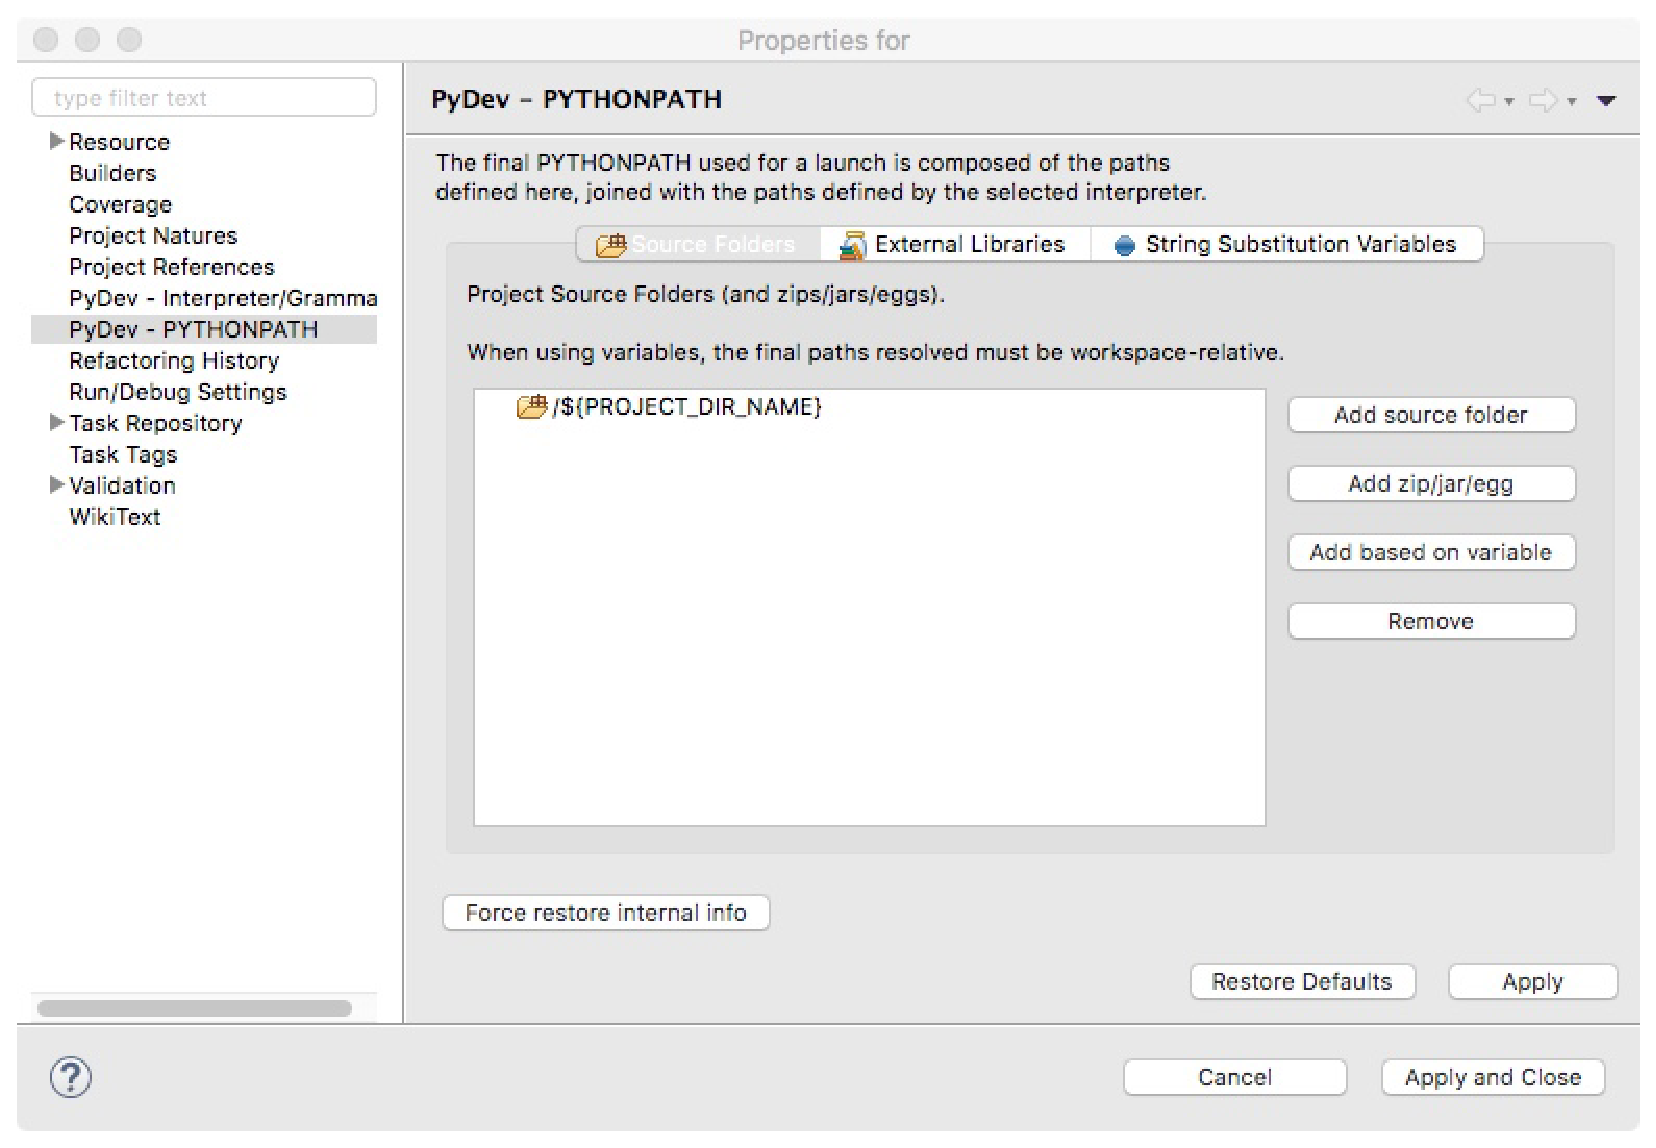
\includegraphics[height=0.45\textwidth]{imagenes/pythonpath}
\end{center}
\caption{Propiedades del proyecto Eclipse para especificar PYTHONPATH}
\label{fig:pythonpath}
\end{figure}

Existe alguna posibilidad adicional después de las anteriores para hacer otro intento de localización, pero no se van a tratar aquí. ¿Y si no se encuentra el módulo? Pues se produce una excepción de tipo \texttt{ImportError}.

\subsubsection{Compilación a bytecodes}

Después de localizar el fichero de código fuente (con extensión \texttt{.py}) del módulo que hay que importar, Python compila el código a bytecodes si es necesario. Para determinar si es necesario, se hace una comparación del instante de última modificación del fichero fuente con el del fichero compilado. Si el primero es posterior al segundo, se realiza la compilación del módulo importado. El resultado es un fichero con extensión \texttt{.pyc} que queda almacenado en el subdirectorio \texttt{\_\_pycache\_\_} dentro del directorio del proyecto.

Ten en cuenta que la compilación sólo se realiza cuando se importa un módulo. Por esta razón, normalmente no verás un fichero \texttt{.pyc} para el módulo principal, a menos que sea importado en otro sitio. ¿Significa esto que el módulo principal no se compila? No, también se compila, pero se hace cada vez que se ejecuta y sus bytecodes no se guardan en ningún sitio, sino que son desechados al finalizar el programa. Conviene que el módulo principal sea lo más pequeño posible para acelerar la ejecución del programa.

\subsubsection{Ejecución del módulo importado}

Hay un último paso en la importación de un módulo: su ejecución. Aquí tienes una buena razón para entender que la importación de módulos de Python no tiene mucho que ver con la directiva de precompilación \texttt{\#include} de C. 

Podemos distinguir dos tipos de código dentro de un módulo: definiciones de funciones y código de \emph{primer nivel}. Las funciones se declaran, como ya hemos visto, con la palabra clave \texttt{def}. En cierta forma podemos considerar que estas declaraciones se \emph{ejecutan} al cargar un módulo en el sentido de que las funciones quedan disponibles para su uso en el módulo que realiza la importación. En cuanto al código de \emph{primer nivel}, se trata de código Python del módulo importado que no forma parte de la definición de funciones. Podríamos considerar que esto de \emph{primer nivel} tiene que ver con el nivel de indentación inicial. Por ejemplo, la inicialización de variables o la típica sentencia \texttt{if \_\_name\_\_ == \_\_main\_\_:} etc., es un caso de código de \emph{primer nivel} de un módulo. Este código se ejecuta al importar el módulo, indistintamente de si se usa \texttt{import} o \texttt{from}.

\subsubsection{Algunas consideraciones más}

Como \texttt{import} y \texttt{from} son sentencias, pueden estar dentro de otras sentencias condicionales. Esto implica que los módulos se puede importar en función de las condiciones que se produzcan durante la ejecución del programa. Por otra parte, es posible realizar varias llamadas de importación de un módulo en el mismo programa. Sólo la primera tendrá como consecuencia la ejecución de los tres pasos que acabamos de ver. Las restantes llamadas de importación reutilizarán el módulo que ya está en memoria.

Cuidado con los nombres de las variables y funciones definidas en un módulo. Si son demasiado generales, como \texttt{x} o \texttt{f}, es posible que tengas montado un buen lío al importar varios módulos en otro si hay coincidencia de nombres y usas \texttt{from}.

\section{Paquetes}

Hasta ahora, sólo hemos visto cómo importar un módulo en otro. Posiblemente, tus primeros desarrollos en Python no necesiten mucho más. Pero, ¿para qué ponerse límites? En el momento en que tus programas Python vayan creciendo, posiblemente necesites una estructura de módulos ordenados en distintos directorios. Aquí es donde viene al rescate el concepto de \emph{paquete} (también lo hemos llamado \emph{librería} en varias ocasiones): un paquete Python no es más que un directorio con una serie de módulos Python, y opcionalmente con subdirectorios (subpaquetes) con más módulos. Sólo hace falta un pequeño detalle para que Python sepa que un directorio es un paquete: debe contener un fichero con el divertido nombre de \texttt{\_\_init\_\_.py}. Ese fichero puede estar vacío, aunque lo normal es que contenga lo siguiente:

\begin{itemize}
\item Código de inicialización del paquete. Por ejemplo, la definición de valores de variables por defecto o la apertura de algún recurso del sistema.
\item Un listado de los módulos que se importan si se usa \texttt{*} en la importación del paquete en una sentencia \texttt{from}. La idea es que quizás no todos los módulos del paquete contienen funciones para ser usadas desde fuera, y sólo queremos que se ejecute la importación de algunos de ellos. El listado se especifica en una variable con el nombre \texttt{\_\_all\_\_}.
\end{itemize}

Supongamos que tenemos un paquete en un directorio llamado \texttt{ordenar}, dentro del cual hay un módulo por cada algoritmo de ordenación: \texttt{bubblesort.py}, \texttt{quicksort.py}, etc. Supongamos que todos estos módulos tienen un método \texttt{sort()} con un argumento que es una lista de enteros, y que el método imprime el resultado de la ordenación.

Dentro del fichero \texttt{\_\_init\_\_.py} del directorio \texttt{ordenar} podemos dar valor a \texttt{\_\_all\_\_} con la lista de módulos que se importan desde el paquete si se usa \texttt{from} con \texttt{*}:
\begin{lstlisting}
# __init__.py del paquete ordenar
__all__ = ["bubblesort","quicksort","mergesort","cocktailsort"]
\end{lstlisting}

A nivel básico, la importación de definiciones de paquetes funciona como con los módulos invididuales, pero ahora usando el nombre del paquete (ruta de directorios) delante:

\begin{lstlisting}
import ordenar.bubblesort
# Uso el método sort del módulo bubblesort
ordenar.bubblesort.sort([5,2,9,34,12])
\end{lstlisting}

El mecanismo de importación realiza la búsqueda del paquete siguiendo el mismo orden de localizaciones posibles que en el caso de los módulos individuales\footnote{Si se importa un paquete contenido dentro de otro paquete, lo importante es localizar al primero, el paquete de más alto nivel, ya que los subpaquetes son subdirectorios del primero.}. Como puedes ver en el código anterior, para invocar al método \texttt{sort} es necesario indicar delante el nombre completo del módulo, incluyendo el nombre del paquete delante. Por esta razón, puede ser conveniente usar \texttt{as} en las sentencias \texttt{import}:

\begin{lstlisting}
import ordenar.bubblesort as bubble
# Uso el método sort del módulo bubblesort renombrado como bubble
bubble.sort([5,2,9,34,12])
\end{lstlisting}

También podemos realizar la importación de un paquete usando la sentencia \texttt{from}:

\begin{lstlisting}
from ordenar import bubblesort
# Uso el método sort del módulo bubblesort
bubblesort.sort([5,2,9,34,12])
\end{lstlisting}

Y si queremos afinar mucho, podemos indicar específicamente el método que queremos usar:

\begin{lstlisting}
from ordenar.bubblesort import sort
# Uso el método sort del módulo bubblesort
sort([5,2,9,34,12])
\end{lstlisting}

Por el contrario, si no tenemos claro qué queremos usar de un paquete, siempre se puede usar una importación a lo salvaje:

\begin{lstlisting}
from ordenar import *
# Uso el método sort del módulo mergesort
mergesort.sort([5,2,9,34,12])
\end{lstlisting}

Observa que, en este último caso, tienes que indicar el módulo delante del método \texttt{sort}	que quieres usar, ya que se han importado todos los módulos indicados en la lista \texttt{\_\_all\_\_} o, en caso de que no esté definida, todos los módulos del paquete.


\subsection{Creación de paquetes en Eclipse}

En la sección \ref{sec:programa_basico} te indicamos cómo se puede crear un módulo dentro de Eclipse. Si le vuelves a echar un vistazo verás que, en el tercer paso, dejamos vacío el campo \texttt{package}. No hace falta ser un genio para darse cuenta de que, si indicamos un nombre de paquete, Eclipse va a crear el módulo dentro de un subdirectorio con el nombre del paquete. Ese subdirectorio se crea en el directorio del proyecto, dentro del \emph{workspace} de Eclipse. Si es el primer módulo de ese paquete, el subdirectorio se crea en ese momento. Si no, simplemente se añade el nuevo módulo.

Existe también la posibilidad de crear un paquete vacío, usando la opción \emph{PyDev Package} dentro del menú \emph{File}, opción \emph{New}.

\subsection{Gestión de paquetes con \texttt{pip}}

Si todo fue correctamente durante la instalación de Python (sección \ref{sec:instalacion}), desde la línea de comandos de tu sistema tendrás la posibilidad de ejecutar el comando \texttt{pip} (podrías necesitar tener permisos de administrador para hacerlo). Es la herramienta básica para acceder al \emph{Python Package Index} (PyPI), el repositorio de paquetes para el lenguaje Python que actualmente cuenta con casi 150000 proyectos\footnote{Puedes acceder a un buscador de paquetes del repositorio en \url{https://pypi.org/}.}.

Lo primero que puede resultar conveniente es actualizar la propia herramienta \texttt{pip} para estar seguros de que tenemos la última versión. Necesitamos usar un comando que es todo un homenaje a la recursión: 

\begin{lstlisting}
pip install --upgrade pip
\end{lstlisting}

Supongamos que, tras buscar un rato en Google, hemos localizado un paquete para reconocimiento de voz que nos interesa usar. El nombre del paquete es \texttt{SpeechRecognition}. Sabiendo el nombre del paquete, la forma de instalarlo es realmente sencilla:

\begin{lstlisting}
pip install SpeechRecognition
\end{lstlisting}

Aparecerá una barra que muestra el progreso de la descarga, y en poco tiempo tendremos instalado el paquete en el equipo. Si eres un poco maniático y quieres tener un control exhaustivo de qué ficheros contiene el paquete que se ha instalado, y exactamente dónde se encuentran, no hay problema, se lo preguntamos a \texttt{pip}:

\begin{lstlisting}
pip show --files SpeechRecognition
\end{lstlisting}

Para saber cuáles son los paquetes que tenemos instalados mediante \texttt{pip}, podemos solicitar un listado de la siguiente forma:

\begin{lstlisting}
pip list
\end{lstlisting}

Junto a cada paquete aparece indicada la versión que tenemos instalada en el sistema. Si quisiéramos ver los paquetes que están desactualizados, podemos hacerlo así:

\begin{lstlisting}
pip list --outdated
\end{lstlisting}

Y si encontramos un paquete desactualizado, podemos actualizarlo a su última versión así:

\begin{lstlisting}
pip install --upgrade paquete
\end{lstlisting}

Desinstalar un paquete es igual de sencillo que instalarlo:

\begin{lstlisting}
pip uninstall paquete
\end{lstlisting}

El comando \texttt{pip} tiene la deferencia de consultarnos si realmente queremos hacer la desinstalación. Si tienes curiosidad, puedes ver que \texttt{pip} se puede hacer el harakiri a sí mismo. 